%-------------------------------------------------------------------------------
% 请勿删除本注释
% Free Response Question 1
%
% 指引:
% 如在小问之前有通用问题描述,请放置于此
%-------------------------------------------------------------------------------
\begin{figure}[H]
\centering
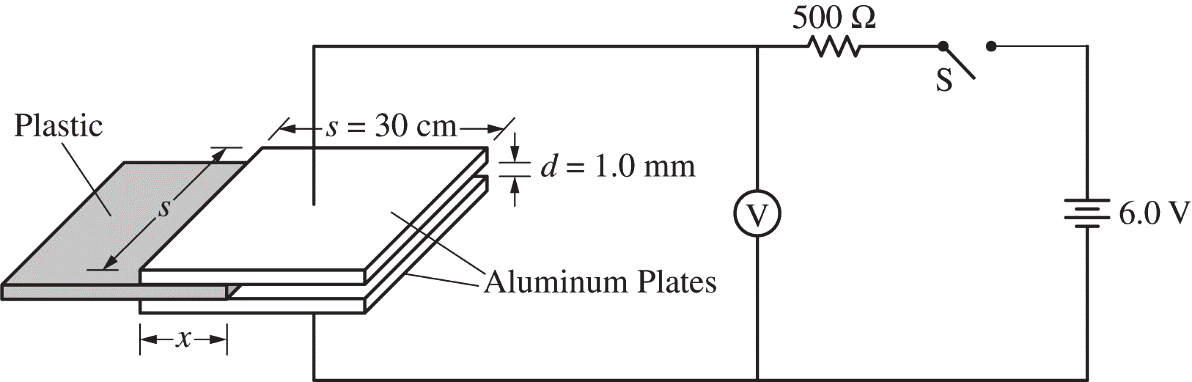
\includegraphics[scale=0.3]{images/img-018-032.png}
\end{figure}

\question
Students design an experiment to determine the unknown dielectric constant $\kappa$ of a plastic material. A capacitor is created using two square aluminum plates of side length $s=30 \mathrm{~cm}$ that are separated by a distance $d=1.0 \mathrm{~mm}$. This capacitor is placed in a circuit with an ideal $6.0$-volt battery, a resistor of resistance $R=500 \Omega$, voltmeter $\mathrm{V}$, and an open switch $\mathrm{S}$, as shown above. A $1.0 \mathrm{~mm}$ thick piece of plastic is inserted between the aluminum plates. The distance $x$ that the plastic is inserted between the plates can be varied, and the voltmeter is used to measure the potential difference $V_{C}$ across the capacitor. The switch is closed, and readings from the voltmeter are recorded as a function of time $t$. The data are plotted to create the graph shown below. % 请删除并替换本行,与上一行 \question 之间不要留空行

\begin{figure}[H]
\centering
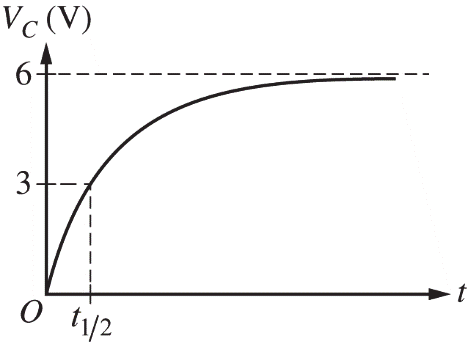
\includegraphics[scale=0.3]{images/img-018-033.png}
\end{figure}

The time $t_{1 / 2}$ shown above is the time for the capacitor to charge to half the potential difference of the battery.

\begin{parts}

%-------------------------------------------------------------------------------
% 请勿删除本注释
% Part (a)
%
% 指引:
% 如在小问之前有通用问题描述,请放置于此
%-------------------------------------------------------------------------------

\part
The potential difference across the capacitor as a function of time is modeled by the equation $V_{C}=V_{\mathrm{MAX}}\left(1-e^{-t / R C}\right)$, where $V_{\mathrm{MAX}}=6 \mathrm{~V}$. Derive an expression for the capacitance $C$ of the capacitor. Express your answer in terms of $t_{1 / 2}, R$, and physical constants, as appropriate. % 请删除并替换本行,与上一行 \part 之间不要留空行

%-------------------------------------------------------------------------------
% 请勿删除本注释
% Part (b)
%
% 指引:
% 如在小问之前有通用问题描述,请放置于此
%-------------------------------------------------------------------------------
The data for $x$ and $t_{1 / 2}$ are recorded for several trials and the value of $C$ for each trial is calculated. The results are shown in the chart below.

\begin{table}[H]
\centering
\begin{tabular}{|l|l|l|l|l|l|}
\hline$x(\mathrm{~m})$ & $0.050$ & $0.10$ & $0.15$ & $0.20$ & $0.25$ \\
\hline$t_{1 / 2}(\mu \mathrm{s})$ & $0.44$ & $0.63$ & $0.75$ & $0.88$ & $1.10$ \\
\hline$C(\mathrm{nF})$ & $1.27$ & $1.82$ & $2.16$ & $2.54$ & $3.17$ \\
\hline
\end{tabular}
\end{table}



\part
Plot the experimental value of the capacitance $C$ as a function of the distance $x$ on the graph below. Clearly scale and label all axes, including units if appropriate. Draw a straight line that best represents the data. % 请删除并替换本行,与上一行 \part 之间不要留空行

\begin{figure}[H]
\centering

\includegraphics[scale=0.3]{images/img-019-034.png}
\end{figure}

%-------------------------------------------------------------------------------
% 请勿删除本注释
% Part (c)
%
% 指引:
% 如在小问之前有通用问题描述,请放置于此
%-------------------------------------------------------------------------------

\part
The capacitor in the lab can be treated as two capacitors in parallel, one with the dielectric and one with air between the plates. Show that the capacitance can be expressed as $C=\frac{\varepsilon_{0} s}{d}(s+x(\kappa-1))$. % 请删除并替换本行,与上一行 \part 之间不要留空行

%-------------------------------------------------------------------------------
% 请勿删除本注释
% Part (d)
%
% 指引:
% 如在小问之前有通用问题描述,请放置于此
%-------------------------------------------------------------------------------

\part
Using the graph from part (b), calculate the value of the dielectric constant $\kappa$. % 请删除并替换本行,与上一行 \part 之间不要留空行

%-------------------------------------------------------------------------------
% 请勿删除本注释
% Part (e)
%
% 指引:
% 如在小问之前有通用问题描述,请放置于此
%-------------------------------------------------------------------------------

\part
The students now want to verify the value for the permittivity constant, $\varepsilon_{0}$. Using the graph from part (b), calculate an experimental value for $\varepsilon_{0}$. % 请删除并替换本行,与上一行 \part 之间不要留空行

%-------------------------------------------------------------------------------
% 请勿删除本注释
% Part (f)
%
% 指引:
% 如在小问之前有通用问题描述,请放置于此
%-------------------------------------------------------------------------------

\part
Assume the value found in part (e) is higher than the accepted value for the permittivity constant. State one possible physical reason for this error and explain how it could have caused this error. % 请删除并替换本行,与上一行 \part 之间不要留空行

\end{parts}
